%=========================================================

% Here you can choose to compile with or without solutions.
% However, this definition is ignored if you use any
% command from the `Makefile`.
\providecommand{\withSol}{\iftrue}

%=========================================================

\documentclass
[twoside,german,colorbacktitle,accentcolor=tud9c]
{tudexercise}

\usepackage[T1]{fontenc}
\usepackage[utf8]{inputenc}
\usepackage[ngerman]{babel}
\usepackage{amstext}
\usepackage{amsmath}
\usepackage{graphicx}
%\usepackage{setspace}
\usepackage{multicol}
\usepackage{mathtools}
\usepackage{dsfont}
\usepackage{units}
%\usepackage{subfigure}
\usepackage{color}
\usepackage{booktabs}
\usepackage{fancyref}
\usepackage{gensymb}
\usepackage{tikz}
\usetikzlibrary{shapes.misc} 
\usepackage[verbose]{placeins}%Floatbarrier

%=========================================================


\setcounter{section}{2}
%=========================================================

\newcommand{\grp}{F}

%=========================================================


\begin{document}

\title{GDV 2 -- Theorie Übung \arabic{section}}
\subtitle{Sommer Semester 2019}
\subsubtitle{Übungsgruppe \grp{}}

\maketitle

%=========================================================



\begin{examheader}
	\textmb{GDV 1 - Theorie Übung \arabic{section} | Gruppe \grp{}}\\
	\begin{tabular}{l l l l l}
		Moritz Fuchs	& Alexander Jäger	& Amon Ditzinger	& John Kalkhoff	\\
	\end{tabular}
\end{examheader} 


%=========================================================
% Anpassung an Aufgabenstellung
\renewcommand\thesubsection{Aufgabe \arabic{subsection}}
\renewcommand\thesubsubsection{\alph{subsubsection})}

%=========================================================
\FloatBarrier
\newif\ifvimbug
\vimbugfalse

\ifvimbug
\begin{document}
\fi


\subsection{Interpolation in verschiedenen Darstellungsformen (5 Punkte)}
\subsubsection{1 Punkt}
$Va = P$\\
\\
$\begin{pmatrix}
1 & 1 & 1 \\ 
1 & 3 & 9 \\ 
1 & 2 & 4
\end{pmatrix} \begin{pmatrix}
a_{0} \\ 
a_{1} \\ 
a_{2}
\end{pmatrix} = \begin{pmatrix}
0 \\ 
2 \\ 
4
\end{pmatrix} $\\
\\
Mit Gauß:\\
\\
$\begin{pmatrix}
1 & 1 & 1 \\ 
0 & 2 & 8 \\ 
0 & 0 & -1
\end{pmatrix} \begin{pmatrix}
a_{0} \\ 
a_{1} \\ 
a_{2}
\end{pmatrix} = \begin{pmatrix}
0 \\ 
2 \\ 
3
\end{pmatrix} $\\
\\
Daraus folgt \\
$a_{0} = -10 \\
a_{1} = 13 \\
a_{2} = -3$ \\
\\
Und das Polynom $P_{M}(t) = -3t^{2} + 13t - 10$\\
\\
Auswertung weiterer Punkte:
\begin{tabular}[optional Position]{c c c c c c c c c c}
	t & 0 & 0,5 & 1 & 1,5 & 2 & 2,5 & 3 & 3,5 & 4 \\
	P(t) & -10 & -4,25 & 0 & 2,75 & 4 & 3,75 & 2 & -1,25 & -6
\end{tabular}\\
\\
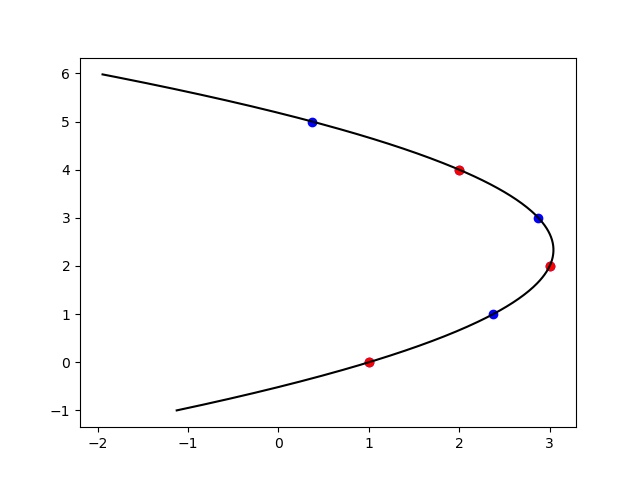
\includegraphics{1a}
\subsubsection{1 Punkt}
$l_{i}(t) = {\displaystyle \prod_{j=0,j \neq i}^{q}} \dfrac{t - t_{j}}{t_{i} - t_{j}}$ \\
\\
$l_{0}(t) = \dfrac{t - 3}{1 - 3} * \dfrac{t - 2}{1 - 2} = \dfrac{1}{2}t^{2} - \dfrac{5}{2}t + 3$ \\
\\
$l_{1}(t) = \dfrac{t - 1}{3 - 1} * \dfrac{t - 2}{3 - 2} = \dfrac{1}{2}t^{2} - \dfrac{3}{2}t + 1$ \\
\\
$l_{2}(t) = \dfrac{t - 1}{2 - 1} * \dfrac{t - 3}{2 - 3} = -t^{2} + 4t - 3$ \\
\\
$P_{L}(t) = {\displaystyle \sum_{i=0}^{q}} l_{i}(t)P_{i} = -3t^{2} + 13t - 10$\\
\\
Offensichtlich sind $P_{M}(t)$ und $P_{L}(t)$ identisch.
\subsubsection{1 Punkt}
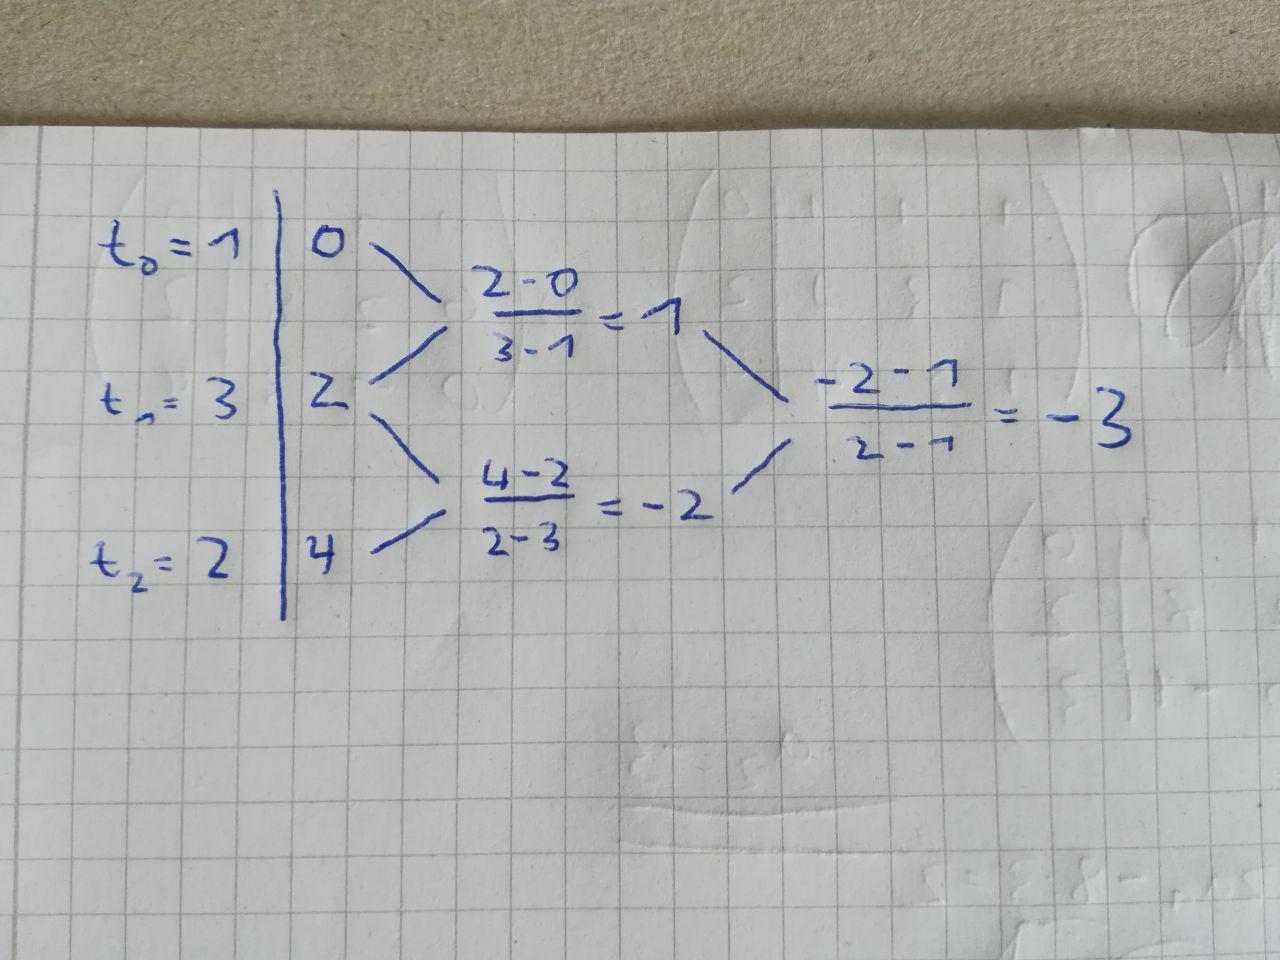
\includegraphics[scale=0.3]{1c}
\\
\\
$P_{N}(t) = 0 + 1(t - t_{0}) - 3(t - t_{0})(t - t_{1}) = t - 1 - 3(t - 1)(t - 3) = -3t^{2} + 13t - 10$\\
Das Polynom $P_{N}(t)$ ist identisch $P_{M}(t)$ und $P_{L}(t)$.
\subsubsection{2 Punkte}
Die Newton-Darstellung lässt sich am einfachsten erweitern, da man dem Dreiecksschema ohne viel Aufwand eine neue Stützstelle hinzufügen kann. \\
\\
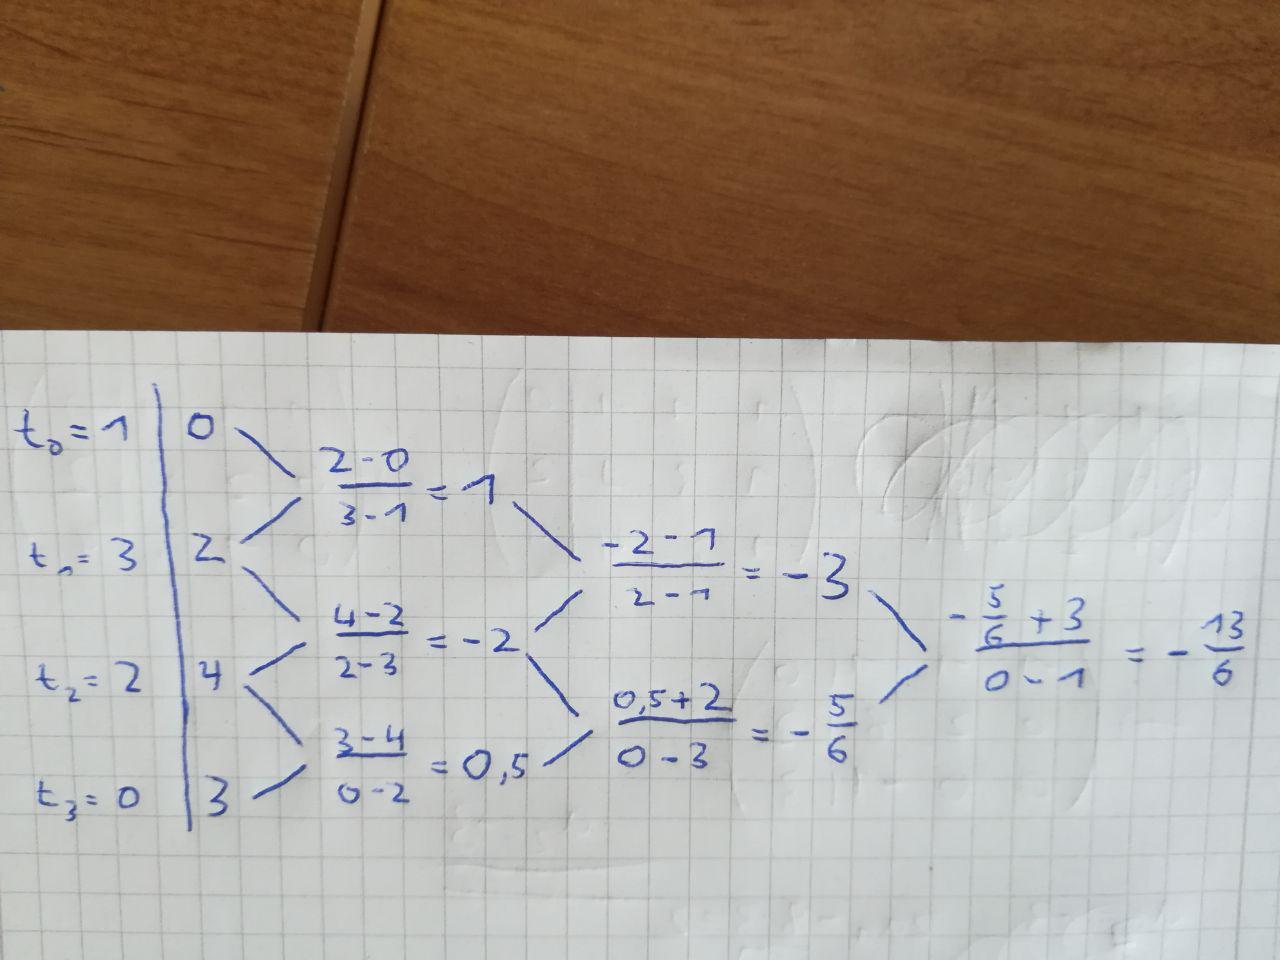
\includegraphics[scale=0.3]{1d}\\
\\
\\
$P_{N}(t) = -3t^{2} + 13t - 10 - \dfrac{13}{6}(t - 1)(t - 3)(t-2) = -\dfrac{13}{6}t^{3} + 10t^{2} - \dfrac{65}{6}t + 3$


\FloatBarrier
\newif\ifvimbug
\vimbugfalse

\ifvimbug
\begin{document}
\fi


\subsection{Bernstein-Bézier-Tensorprodukte (7 Punkte)}
\subsubsection{3 Punkte}
Wir wenden de Casteljau an mit $v=\frac{3}{4}$ und $\lambda= \frac{1}{4}$:\\
\begin{tikzpicture}[grow=left,
level 1/.style={sibling distance=15mm},edge from parent/.style={-,draw},>=latex, level 3/.style={edge from child/.style={->,draw},sibling distance=15mm}]

\node[root] {$\begin{pmatrix}-2.125\\ 2.5625\\5.4375\end{pmatrix}$}
     child {node[level 2] (c1) {$\begin{pmatrix}-1\\2\\3\end{pmatrix}$}
           child {node[level 2] (c11) {$\begin{pmatrix}-1\\2\\0\end{pmatrix}$}}
       child {node[level 2] (c21) {}}
       }
 child {node[level 2] (c2) {$\begin{pmatrix}-2.5\\2.75\\6.25\end{pmatrix}$}
	child {node[level 2] (c21) {$\begin{pmatrix}-1\\2\\4\end{pmatrix}$}}
       child {node[level 2] (c22) {$\begin{pmatrix}-3\\3\\7\end{pmatrix}$}}
       };
       \draw[-, draw] (c21) -- (c2);
\end{tikzpicture}\\

\begin{tikzpicture}[grow=left,
level 1/.style={sibling distance=15mm},edge from parent/.style={-,draw},>=latex, level 3/.style={edge from child/.style={->,draw},sibling distance=15mm}]

\node[root] {$\begin{pmatrix}3\\3.4375\\4.875 \end{pmatrix}$}
     child {node[level 2] (c1) {$\begin{pmatrix}3\\2.5\\3 \end{pmatrix}$}
           child {node[level 2] (c11) {$\begin{pmatrix}3\\1\\0\end{pmatrix}$}}
       child {node[level 2] (c21) {}}
       }
 child {node[level 2] (c2) {$\begin{pmatrix}3\\3.75\\5.5 \end{pmatrix}$}
	child {node[level 2] (c21) {$\begin{pmatrix}3\\3\\4\end{pmatrix}$}}
       child {node[level 2] (c22) {$\begin{pmatrix}3\\4\\6\end{pmatrix}$}}
       };
       \draw[-, draw] (c21) -- (c2);
\end{tikzpicture}\\

\begin{tikzpicture}[grow=left,
level 1/.style={sibling distance=15mm},edge from parent/.style={-,draw},>=latex, level 3/.style={edge from child/.style={->,draw},sibling distance=15mm}]

\node[root] {$\begin{pmatrix}6.5\\1.375\\6.5625 \end{pmatrix}$}
     child {node[level 2] (c1) {$\begin{pmatrix}7.25\\1.75\\3\end{pmatrix}$}
           child {node[level 2] (c11) {$\begin{pmatrix}8\\1\\0\end{pmatrix}$}}
       child {node[level 2] (c21) {}}
       }
 child {node[level 2] (c2) {$\begin{pmatrix}6.25\\1.25\\7.75\end{pmatrix}$}
	child {node[level 2] (c21) {$\begin{pmatrix}7\\2\\4\end{pmatrix}$}}
       child {node[level 2] (c22) {$\begin{pmatrix}6\\1\\9\end{pmatrix}$}}
       };
       \draw[-, draw] (c21) -- (c2);
\end{tikzpicture}\\
Wir wenden de Casteljau an mit $u=\frac{1}{4}$ und $\lambda= \frac{3}{4}$:\\
\begin{tikzpicture}[grow=left,
level 1/.style={sibling distance=15mm},edge from parent/.style={-,draw},>=latex, level 3/.style={edge from child/.style={->,draw},sibling distance=15mm}]

\node[root] {$\begin{pmatrix}0.3359375\\2.81640625\\5.296875   \end{pmatrix}$}
     child {node[level 2] (c1) {$\begin{pmatrix}-0.84375\\2.78125\\5.296875\end{pmatrix}$}
           child {node[level 2] (c11) {$\begin{pmatrix}-2.125\\ 2.5625\\5.4375\end{pmatrix}$}}
       child {node[level 2] (c21) {}}
       }
 child {node[level 2] (c2) {$\begin{pmatrix}3.875\\2.921875\\5.296875\end{pmatrix}$}
	child {node[level 2] (c21) {$\begin{pmatrix}3\\3.4375\\4.875\end{pmatrix}$}}
       child {node[level 2] (c22) {$\begin{pmatrix}6.5\\1.375\\6.5625 \end{pmatrix}$}}
       };
       \draw[-, draw] (c21) -- (c2);
\end{tikzpicture}\\
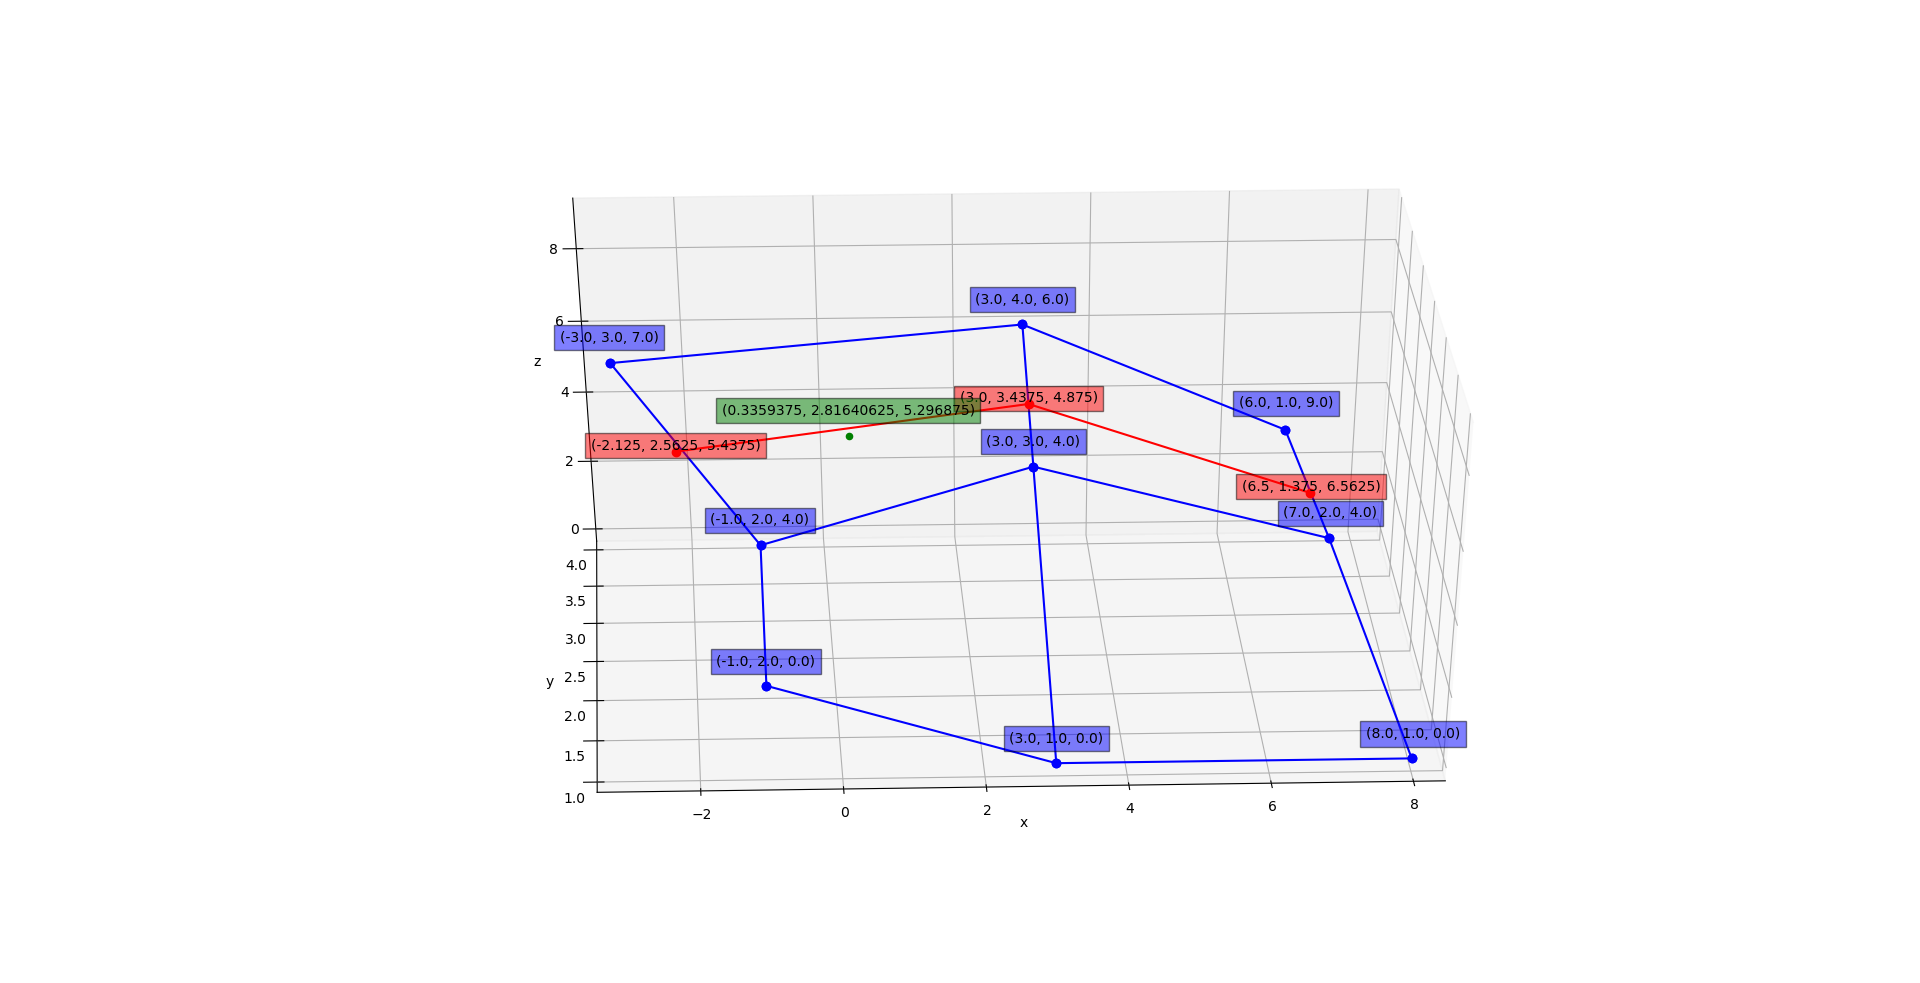
\includegraphics[width=0.9\textwidth]{2_a.png}
\subsubsection{2 Punkte}
hierzu bestimmen wir die kontrollpunkte an den Intervallsgrenzen, wie in Aufgabeteil a. in der grafik sind ist die Neue untereilung eingezeichnet.\\ 
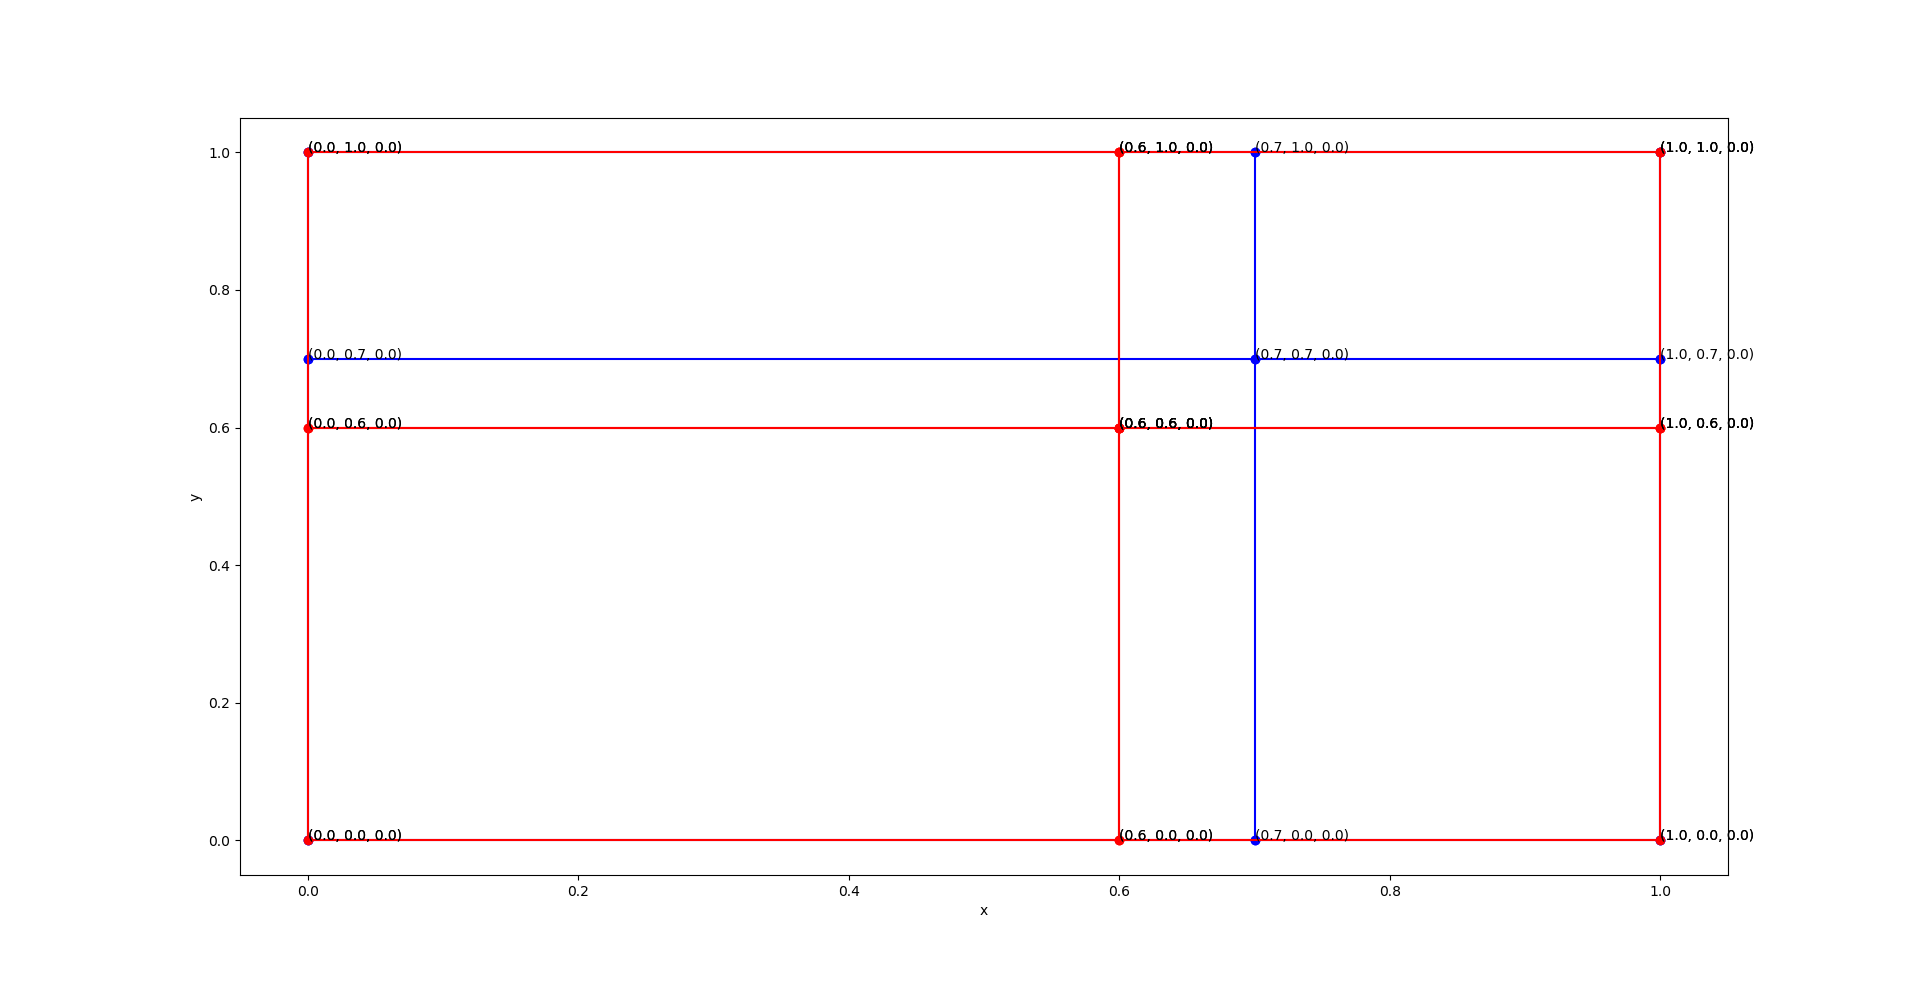
\includegraphics[width=0.9\textwidth]{2_b.png}
\subsubsection{2 Punkte}
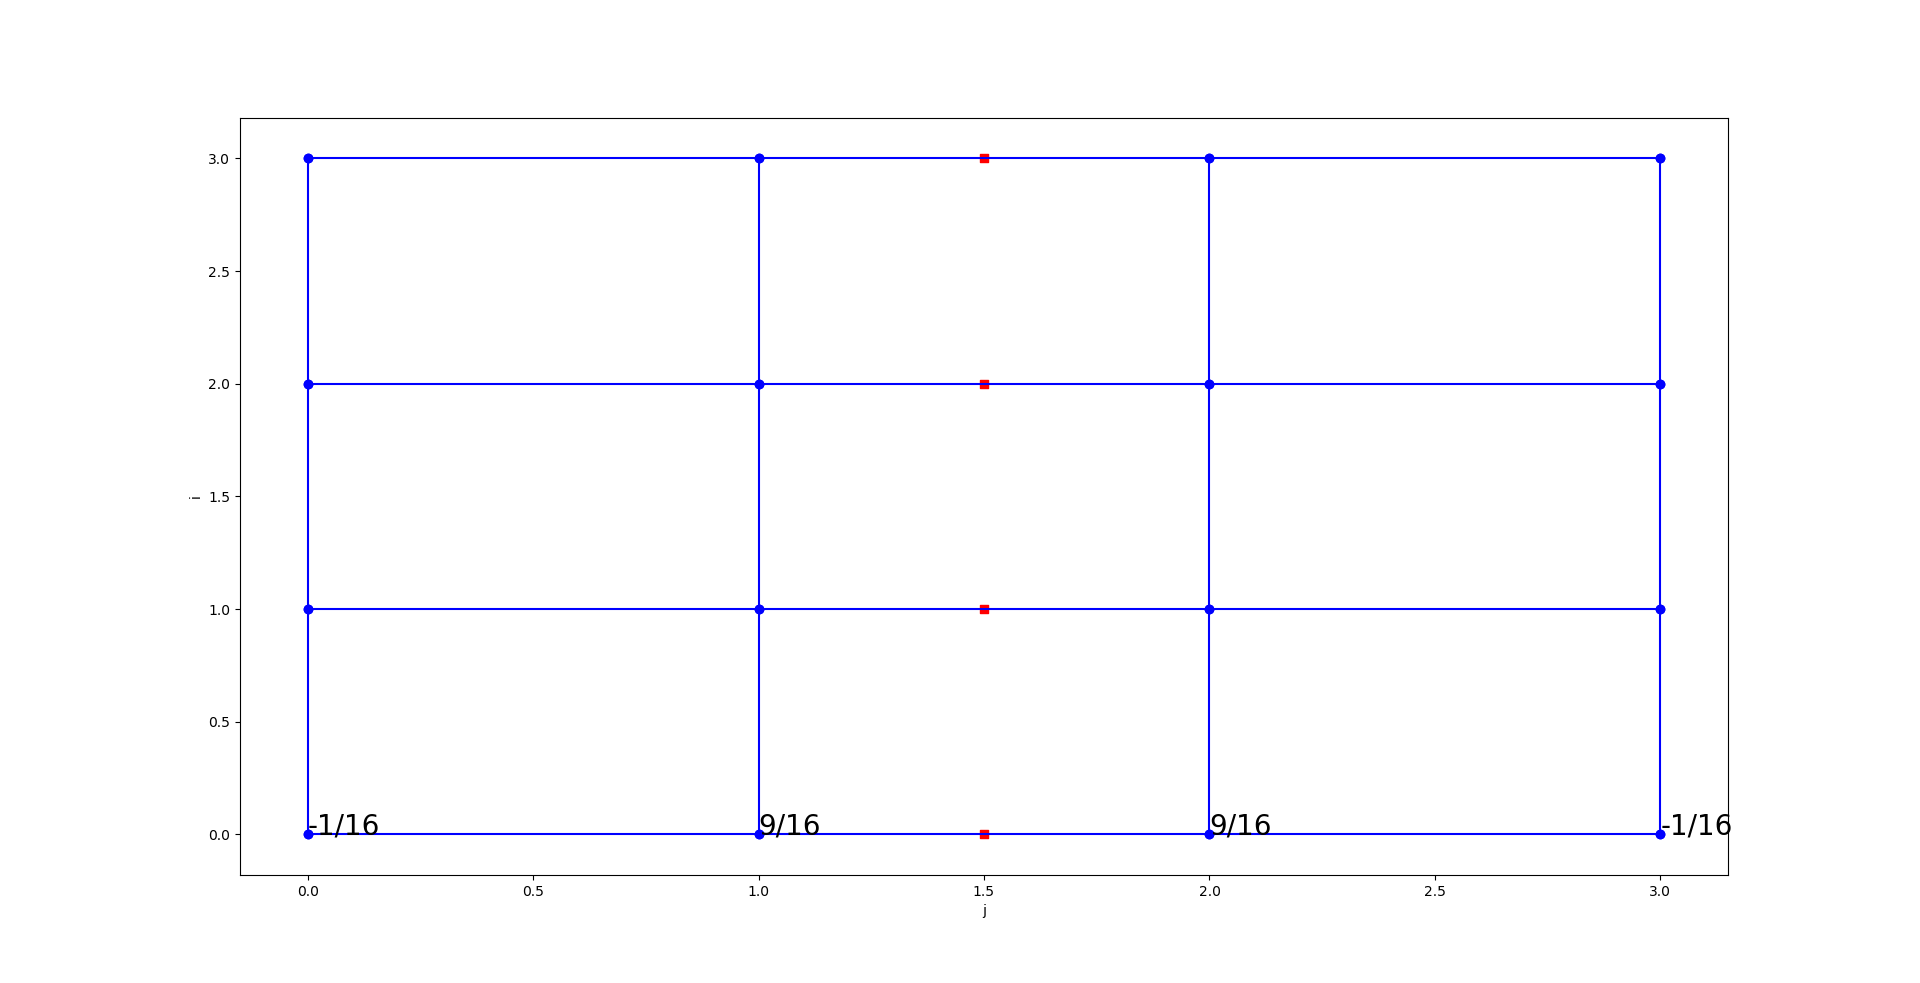
\includegraphics[width=0.5\textwidth]{2_c_P1.png}\\
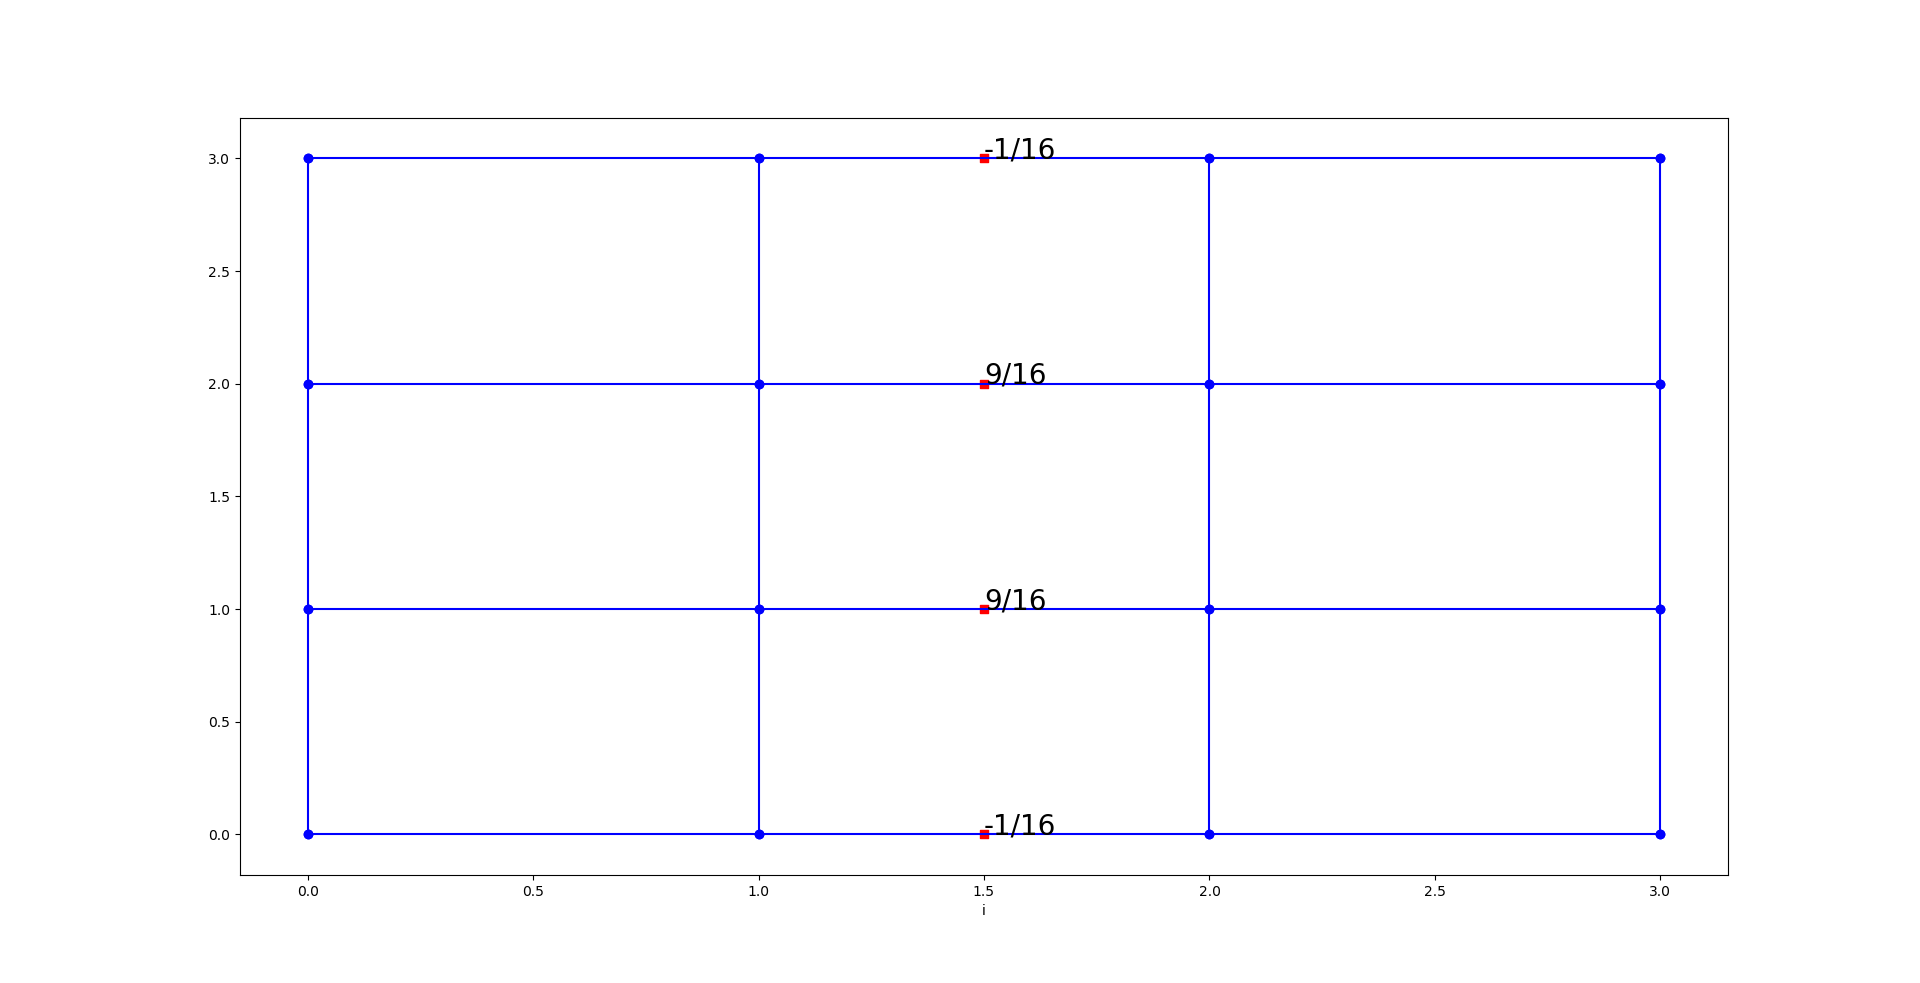
\includegraphics[width=0.5\textwidth]{2_c_P2.png}\\
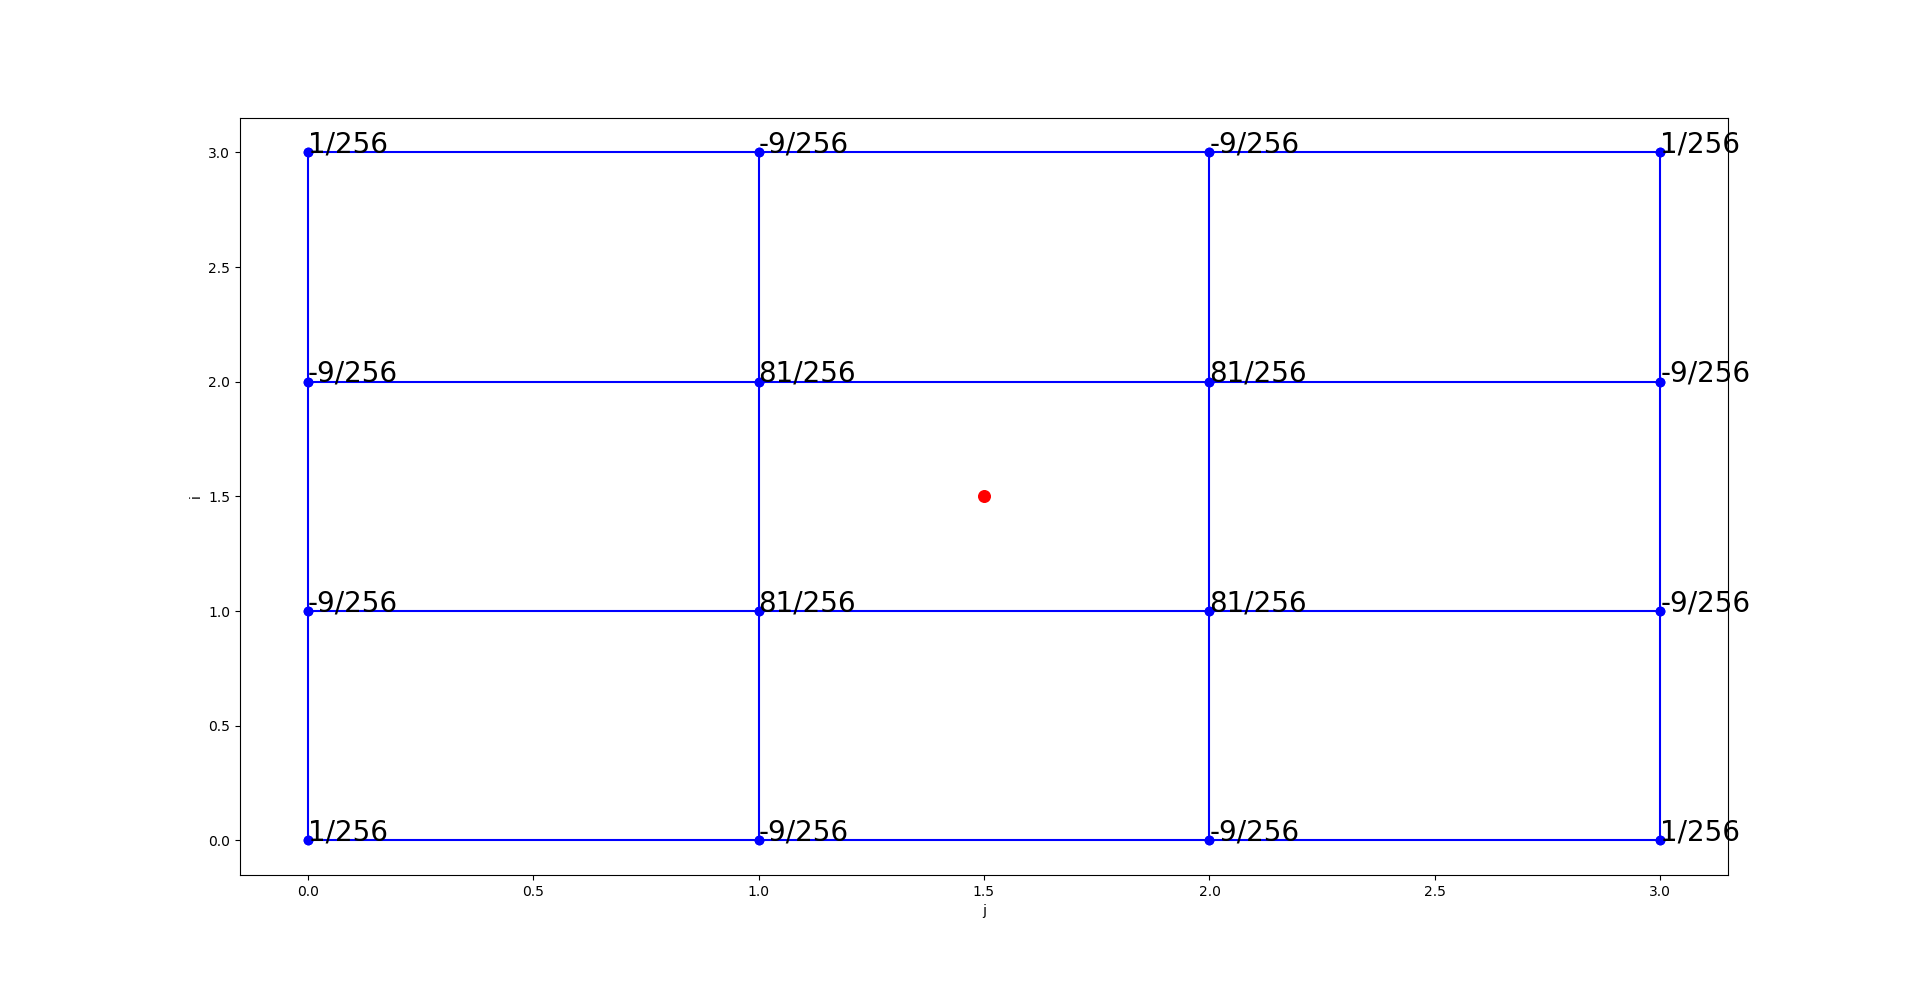
\includegraphics[width=0.5\textwidth]{2_c_P3.png}

\FloatBarrier
\newif\ifvimbug
\vimbugfalse

\ifvimbug
\begin{document}
\fi


\subsection{Approximation in Bernstein-Bézier-Darstellung (4 Punkte)}
\subsubsection{1 Punkt}
\subsubsection{1 Punkt}
\begin{center}
  \makebox[\textwidth]{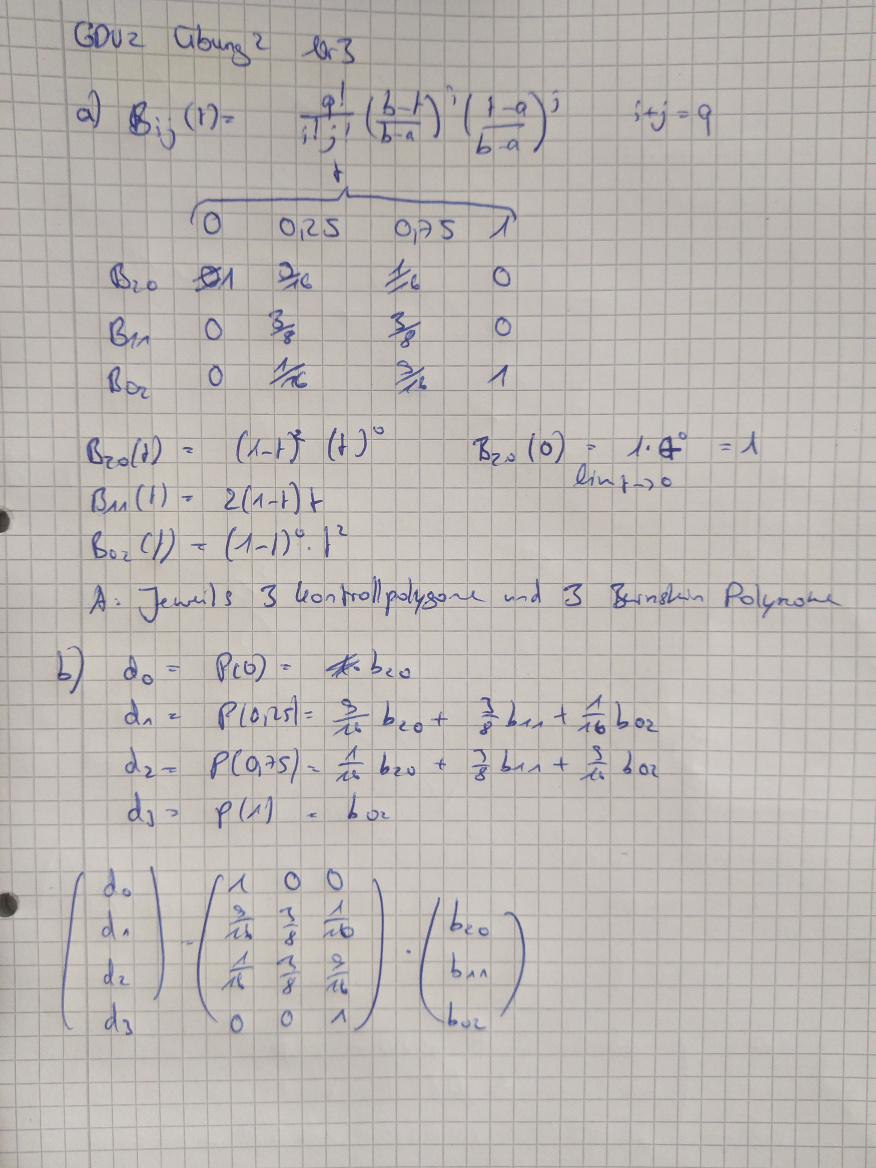
\includegraphics[width=\textwidth]{3ab}}
\end{center}


\subsubsection{1 Punkt}
\begin{center}
  \makebox[\textwidth]{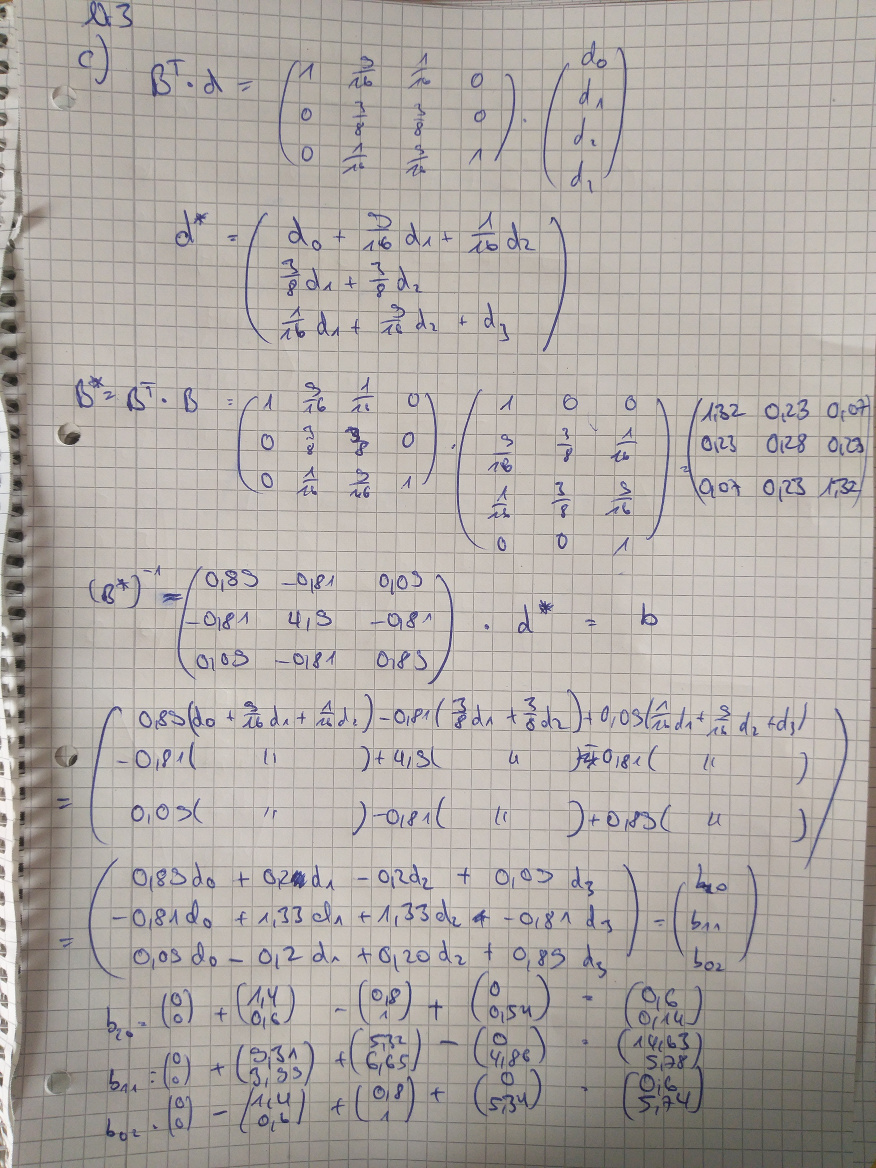
\includegraphics[width=\textwidth]{3c}}
\end{center}
\subsubsection{1 Punkt}
In Rot die Datenpunkte.
In Blau die Kontrollpunkte
und der Verlauf der Approximation in schwarz.\\
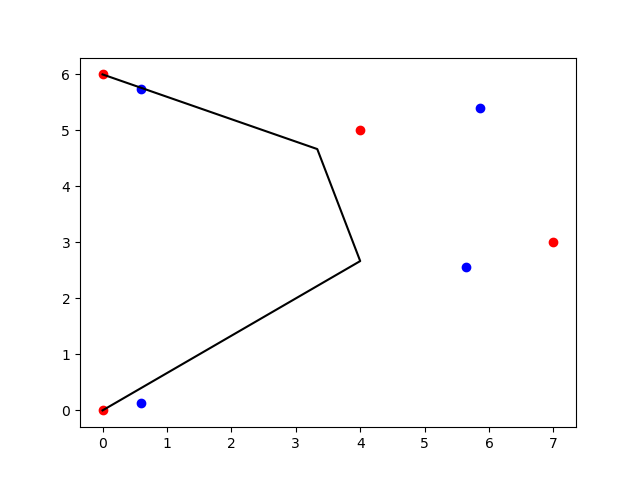
\includegraphics[width=\textwidth]{3d}


\FloatBarrier
\newif\ifvimbug
\vimbugfalse

\ifvimbug
\begin{document}
\fi


\subsection{B-Splines vom Grad 2 (6 Punkte)}
\subsubsection{1 Punkt}

\subsubsection{1 Punkt}

\subsubsection{1 Punkt}

\subsubsection{1 Punkt}

\subsubsection{2 Punkte}


%=========================================================

\end{document}
